\chapter{State of the Art}
Im folgenden Kapitel werden die Features vom MRP-Planungssystem sowie der EWS Schnittstelle dargestellt.

\section{EWS API}
Die Java Exchange Web Services (EWS) Application Programming Interface (API) ist eine Schnittstelle, die von Microsoft bereitgestellt wird, welche die Kommunikation mit einen Microsoft Exchange-Server zulässt. Die API kann mit Java, C\# angesteuert werden und beinhaltet einen umfangreichen Funkionskatalog um die verschiedenen Funktionen in Microsoft Outlook anzusteuern. Diese Funktionen dienen zur Verwaltung von Emails, Kontakten, Aufgaben, Terminen, Kalendern sowie Rechten. Die API wurde entwickelt um programmgesteuerte Abfragen und Aufgaben mit Hilfe eines Microsoft Outlookservers zu realisieren. Sie unterstützt synchrone sowie asynchrone Abfragen und Anfragen an den Server, die zur Abfrage von Verfügbarkeiten und Benutzerrechten sowie von Microsoft Outlookelementen und Ordnern dienen. Weiters kann mit Hilfe der API gefiltert und gesucht werden, weiters lässt die EWS API einen Mehrbenutzerbetrieb zu.\cite{ews2016}
\subsubsection{HyperText Transfer Protocol und HyperText Transfer Protocol Secure}
Das Internetprotokoll HyperText Transfer Protocol (HTTP) beschreibt die zustandslose Übertragung von Internetdaten. Die Übertragung läuft über die Webmethoden GET, PUT und POST. HTTP verwendet die Standardports, welche in der Transmission Control Protocol (TCP)-Richtlinie definiert worden sind.\\ HyperText Transfer Protocol Secure (HTTPS) stellt die sichere Verbindung von HTTP dar, wobei die Verschlüsselung über Secure Socket Layer (SSL) erfolgt. Webseiten werden mittels HyperText Markup Language (HTML), JavaScript und Personal Home Page (PHP) angesteuert, wobei die Daten mit Extensible Markup Language (XML) und JavaScript Object Notation (JSON) übertragen werden.\cite{ews2016,w3c}
\subsection{Funktionen}
\subsubsection{Exchange Service}
Der Exchange Service ist der zentrale Service, welcher Aufgaben verarbeitet und in Verbindung mit dem HTTP(S) Protokoll den Exchange-Server ansteuert. Dieser Service stellt die Verbindung mit dem Server mittels Benutzername, Passwort, Serveradresse her. Außerdem sind zusätzliche Informationen zur Serverversion und Übertragungsart gespeichert. Um die Kommunikation mit dem Server zu ermöglichen, muss die EWS Funktion freigeschaltet sein.\cite{ews2016}
\subsubsection{Items und Folder}
Die Funktionen der EWS API funktionieren nach dem Prinzip der Eindeutigkeit. Dies bedeutet, dass jeder Ordner, jedes Mail und jeder Termin seine eigene ID besitzt, welche vom Server festgelegt wird. Dabei gibt es keine Einschränkung, da jedes Element über die gleiche Priorität verfügt. Weiters kann mit Hilfe dieser eindeutigen ID jedes gesonderte Element abgerufen und beliebig verändert werden. Die Ordner  verfügen über eine eindeutige ID mit der auf den ganzen Ordner zugegriffen werden kann. Auch besitzen spezielle Ordner wie z.B. der Posteingang sogenannte \textit{WellKnownFolderName}s, welche wie Aliase bzw. Pseudonyme für IDs fungieren.\cite{ews2016}
\subsubsection{Email}
Emails können mit Hilfe der API gesendet und empfangen werden. Dabei besitzt jedes Email einen zugeordneten Ordner. Die Emails werden automatisch versendet sobald sie am Server eingetroffen sind. Auch können Emails von beliebigen Konten abgefragt und verändert werden. Vordefinierte Kategorien ermöglichen eine organisierte Verwaltung. Es können Dateien aus dem lokalen Dateisystem an Emails angehängt werden. Wichtige Emails können per Filter gesucht und gefunden werden sowie Posteingangsregeln erstellt und abgerufen werden. Emails können bei Bedarf in einen Unterordner verschoben werden. \cite{joos2013}
\subsubsection{Termine / Appointments}
Termine können erstellt, abgerufen und gelöscht werden. Sie repräsentieren eine Hauptfunktionalität im Outlook. Jeder Termin beinhaltet Datum, Zeit, Ort sowie Teilnehmer. Die Termine werden in den persönlichen Kalendern abgelegt. Weiters können den Terminen optionale Teilnehmer hinzugefügt werden. Periodisch wiederholende Termine werden als Serientermine hinterlegt. Neben dem Hauptkalender können zusätzliche Kalender erstellt werden. Eine weitere Funktionalität stellt die Abfrage von Verfügbarkeiten dar. Diese liefern in weiterer Folge Terminvorschläge. Dabei wird auch die terminliche sowie räumliche Verfügbarkeit mitgeliefert. \cite{joos2013}

\subsubsection{Tasks}
Ein weitere Funktionalität der API stellen Tasks dar, welche erstellt und abgerufen werden können. Tasks enthalten eine Liste von Aufgaben, welche Personen zugeordnet werden und von diesen abgearbeitet werden. Einzelne Aufgaben können priorisiert und kategorisiert werden.\cite{ews2016}
\subsubsection{Kontakte}
Kontakte stellen neben den Terminen eine wichtige Rolle in der Microsoft Outlookumgebung dar. Die Kontakte werden im Adressbuch verwaltet und können angelegt, abgerufen sowie gelöscht werden. Kontakte können aus vordefinierten Dateien importiert und exportiert werden. Das Adressbuch enthält Kontakte sowie Kontaktgruppen. In den Kontakten sind Namen, Telefonnummern, Emailadressen und persönliche Daten hinterlegt. In dem Adressbuch kann gesucht und gefiltert werden.\cite{joos2013}

\section{Multidimensionales Ressourcen Planning (MRP)}

Das MRP-System ist zur Planung von Krankenhausterminen entwickelt worden. Die Hauptaufgabe von MRP ist es aus gegebenen Ressourcen (Personen, Räume, Geräte, Betten, Materialien) in Verbindung mit Regeln Planungskalender für einzelne Räume zu erstellen. Diese Kalender repräsentieren Operationsplanungen, die eine zentrale Einheit in einem Krankenhausinformationssystem (KIS) darstellen.\\ Ein KIS besteht in erster Linie aus den Zentralkomponenten Organisation, Bettenmanagement, Aufnahme, Entlassung sowie Operationsplanungen. MRP deckt nicht die zentralen Komponenten ab, da sich dieses System nur mit der Planung von Räumen und Terminen mithilfe von Ressourcen beschäftigt. Es übernimmt nicht die Verwaltung des Krankenhauses! \cite{g3mrp,haas2004}
\subsection{Funktionsweise}
Das MRP System generiert aus vorgegebenen Daten geeignete Termine und Pläne für Räume des Krankenhauses. Es werden die benötigten Ressourcen gesammelt und in einer zentralen Datenbank  verwaltet. Aus den Datensätzen werden mittels Ressourcenmanager die Ressourcen zusammengetragen und Appointments generiert. Diese werden dann mit Hilfe des Kapazitätsmanagementtools den verfügbaren Kapazitäten der einzelne Ressourcen zugeordnet und in einer Kalenderansicht dargestellt. \cite{g3mrp}\\
\subsection{Masterdata}
Jedes Feature im MRP-System folgt der selben Struktur. Jedes Feature besteht aus den Teilen API, Component, Datenbank und Service. Dabei wird die Drei-Schichten-Architektur realisiert. Dies bedeutet, dass es drei getrennte Implementierungen hinsichtlich jeder Schicht gibt, welche als eigenständig fungieren. Die unterste Schicht wird als Datenbank-Schicht bezeichnet und ist zuständig für die Verwaltung von persistenten Daten. Die Mittlere Schicht wird als Business-Logik bzw. Verarbeitungsschicht bezeichnet. Diese ruft die Daten von der untersten Schicht ab und leitet sie gegebenenfalls an die oberste Schicht weiter. Es besteht die Möglichkeit für Berechungen und Änderungen der Daten. Die oberste Schicht stellt die Präsentationsschicht dar und ist zuständig für die visuelle Darstellung der Daten. Die 3-Schichten-Architektur hat den Vorteil, dass die Aufgaben der Schichten klar von einander getrennt sind. Weiters gibt es die Component-Service-Implementation, welche aus den Komponenten, Datenbank, Service, und API besteht.\cite{g3r,g3mrp}
\subsubsection{Struktur}
Jedes Feature folgt der Component-Service-Implementation, welche aus folgenden Teilen besteht(siehe Abb. 2.1)\cite{html5,g3r,g3rp,g3mrp}:\\
	\begin{figure}[H]
	\centering
		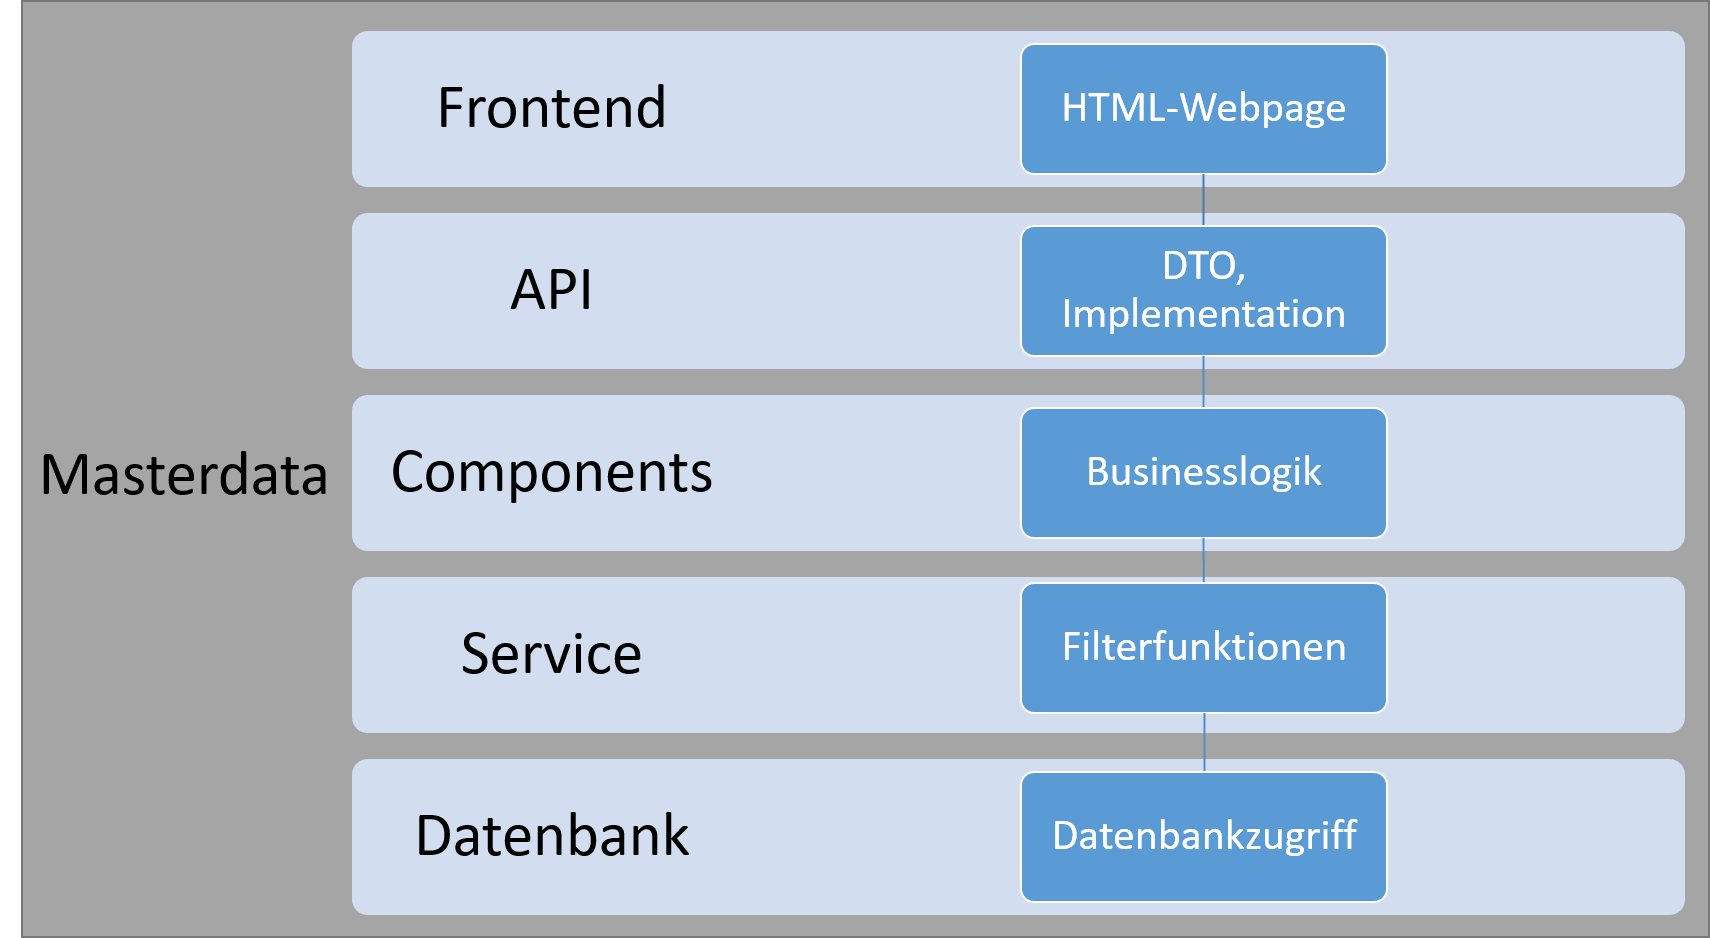
\includegraphics[width=0.8\textwidth]{diagramm1.png}
\caption{Architekturdiagramm}
\end{figure}

 \begin{itemize}
	


\item \textit {Datenbank:} Das Datenbankfeature verwaltet alle Daten in einer Datenbanktechnologie, welche variabel auswählbar ist. Das Speichern und Abrufen von Daten wird über den jeweiligen Datenbanktreiber betrieben, welcher mit einer standardisierten Datenbankansteuerung kommuniziert. Dieser befindet sich innerhalb eines Data Access Object (DAO). Dieses beinhaltet die relevanten Datenbankzugriffsfunktionen und liefert ein Data Transfer Object (DTO).\\
\item \textit{Service:} Der Service erhält Daten von der Datenbank und schickt sie an die Components weiter. Die Services dienen den Components für eine erleichterte Abfragemöglichkeit von Datenobjekten. Weiters benötigen die Services vordefinierte Filterfunktionen. Die Funktionalität der Services gehört der Business-Logik-Schicht an.\\
\item \textit{Components:} Die Components stellen im Feature die Hauptbestandteile dar und sind ein Teil der Businesslogik. Die Components repräsentieren die eigentliche Logik, da in diesen Funktionen die Verarbeitung der Daten erfolgt. Die Components erhalten die Daten aus der Datenbank und wandeln diese in \textit{Data Transfer Objects} um. Die Objekte werden an die API weitergeleitet.\\
\item \textit{API:} Die API ist ein Teil der Businessschicht und stellt die Verbindung zum Frontend da. Die API bekommt die Daten von den Components und wandelt diese in webkonforme Übertragungsobjekte um, welche an das Frontend weitergeleitet werden. Außerdem ist die API zuständig für das Empfangen von Daten aus dem Frontend.\\
\item \textit{Frontend:} Das Frontend repräsentiert die Präsentationssschicht, welche für den jeweiligen Benutzer sichtbar ist. Im Frontend werden die Benutzerinteraktionen verwaltet, Daten zu Transferobjekte umgewandelt und an das Backend gesendet. \\
\item \subsection{Hospital Information System}
Das Hospital Information System (HIS) von CGM wird unter der Produktbezeichnung G3 HIS geführt und besteht aus mehreren Modulen. Die Zentralkomponenten eines KIS sind in diesem System integriert und bilden eine einheitliche Weboberfläche. Diese ist betriebssystemunabhängig und wird in einem vom G3 HIS unterstützten Browser verwendet. Das G3 HIS Projekt umfasst mehrere Projektgruppen, die in die unterschiedlichen Aufgaben (Organisation, Bettenmanagement, Aufnahme, Entlassung, Operationsplanungen) eines Krankenhauses unterteilt sind. Sie bieten eine umfangreiche Konfiguration und Verwaltung der einzelnen Funktionsgruppen bzw. Module an. Die Software stellt die 3. Generation dar und wird ständig weiterentwickelt.
\end{itemize}










